\chapter{Evaluating the solution}

\section{Post-development testing}

\subsection{Test table}

\begin{longtable}{|p{0.02\textwidth}|p{0.2\textwidth}|p{0.25\textwidth}|p{0.25\textwidth}|p{0.1\textwidth}|p{0.06\textwidth}|}
	\hline
	\textbf{\#} & \textbf{Test} & \textbf{Expected Behaviour} & \textbf{Justification} & \textbf{Test Type} & \textbf{Pass?} \\
	\hline
	\endhead
	
	1 & Input item 101 in a 10×10 grid via points entry field & Error message: "Point 101 does not exist in current grid configuration" & Tests error handling for out-of-bounds items to ensure the system validates input before attempting path calculation & Erroneous & X \\
	\hline
	2 & Input "abc" in the points entry field & Error message: "Invalid Input: Please enter valid points" & Validates non-numeric input handling to prevent type errors in the processing logic & Erroneous & X \\
	\hline
	3 & Configure a 0×5 grid using configuration screen & Error message: "Invalid grid dimensions, rows and columns must be at least 1" & Tests boundary validation for minimum grid size to ensure system prevents invalid configurations & Boundary & X\\
	\hline
	4 & Configure a 51×50 grid using configuration screen & Error message: "Invalid grid dimensions. Maximum rows allowed is 100" & Tests upper boundary limits for grid configuration to ensure system prevents excessive resource consumption & Boundary & X\\
	\hline
	5 & Set quantity of ItemID 25 to 0, then attempt to include it in path by entering points "20,25,30" & Point 25 is omitted from pathfinding and an error message is shown & Tests zero-stock validation to ensure the system prevents journeys to zero-inventory locations & Functional & \~{}\\
	\hline
	6 & Set quantity of ItemID 25 to -5 using update quantity function & Error message: "Invalid quantity. Value must be 0 or positive" & Tests negative value validation to ensure database integrity for stock quantities & Erroneous & X\\
	\hline
	7 & Set obstacles to completely block all paths between points 1 and 25 in a 5×5 grid, then attempt pathfinding & Error message: "No path found between the given points" within 5 seconds & Verifies system correctly identifies impossible path scenarios and provides appropriate feedback & Functional & X\\
	\hline
	8 & Enter start or end points (1 or 100) in points field for a 10×10 grid & Error message: "You have inputted a start and/or end point. Please remove it!" & Tests validation logic for preventing the selection of reserved points (start/end) & Functional & X\\
	\hline
	9 & Enter comma-separated points with trailing space "5 10 15 " & Uses existing points and finds a path & Tests parsing robustness for malformed input to ensure the system handles common input errors & Erroneous & X \\
	\hline
	10 & Enter a valid path with points "5,10,15" in a 10×10 grid with all items in stock & System calculates and displays optimal path including points 1,5,10,15,100 within 5 seconds & Tests core pathfinding functionality under normal operating conditions & Functional & X\\
	\hline
	11 & Update quantity of non-existent ItemID 101 in a 10×10 grid & Error message: "Error: ItemID 101 does not exist" & Tests boundary validation for database operations to prevent manipulation of non-existent records & Boundary & X\\
	\hline
	12 & Query information for ItemID 0 & Error message: "No item found" or "ItemID must be at least 1" & Tests lower boundary validation for item query functionality & Boundary & X \\
	\hline
	13 & Configure a 1×1 grid (minimum possible size) & System should create grid with single cell, start and end both at position 1 & Tests minimum boundary case for grid configuration to ensure the system handles edge cases & Boundary & X \\
	\hline
	14 & Configure a 50×50 grid (maximum allowed size) & System should create grid with 2500 cells without freezing or crashing & Tests maximum boundary case for grid configuration to assess system stability under maximum load & Boundary & X \\
	\hline
	15 & Set all intermediate points to have 0 quantity in a 5×5 grid, then attempt pathfinding & Error message indicating all points are unavailable or out of stock & Tests comprehensive validation when all requested points are invalid & Functional & X \\
	\hline
	16 & Create a path where points 5,10,15 are visited, then run again after setting point 10 to quantity 0 & Second run should find alternative path excluding point 10 & Tests system adaptation to changing inventory conditions & Functional & X \\
	\hline
	17 & Save configuration with specific setup to JSON file, then load the same file & System should restore exact grid dimensions, obstacles, and item quantities with 100\% accuracy & Tests data persistence functionality to ensure configurations can be reliably saved and restored & Functional & N/A\\
	\hline
	18 & Load a deliberately corrupted JSON configuration file & Error message indicating invalid configuration file, system should maintain previous state & Tests error handling for data integrity issues to prevent system corruption & Erroneous & N/A \\
	\hline
	19 & Rapidly click the "Find Path" button 10 times in succession & System should ignore additional clicks while processing, without crashing & Tests UI stability under rapid user interaction to ensure the system handles potential race conditions & Stress & X\\
	\hline
	20 & Set obstacles in a pattern forcing a very long path ($>$50 steps) in a 10×10 grid & System should calculate correct path navigating all obstacles within reasonable time ($<$10 seconds) & Tests pathfinding algorithm performance in worst-case scenarios & Performance & X\\
	\hline
	21 & Request path through 20 intermediate points in a 20×20 grid & System should calculate optimal path visiting all points within 10 seconds & Tests algorithm scalability for complex routing scenarios & Performance & X\\
	\hline
	22 & Enter points with mixed spacing "5, 10,15, 20" & System should correctly parse input and calculate path through points 5,10,15,20 & Tests input parsing flexibility to handle various user input formats & Functional & \~{} \\
	\hline
	23 & Use obstacle mode to create a complex maze with only one valid orthogonal path, then request pathfinding & System should find the only valid path through maze & Tests path finding in highly constrained environments & Functional & X \\
	\hline
	24 & Click on a grid cell with quantity 5, verify information displayed & Dialogue should show correct ItemID, row, column, and quantity (5) & Tests item information display functionality & Functional & \~{} \\
	\hline
	25 & Set ItemID 42 to quantity 0 and verify its visual representation in grid & Cell should be highlighted in red colour in the visualisation & Tests correct visual indication of out-of-stock items & Functional & X\\
	\hline
	26 & Update quantity of an item to 1, then traverse path through this item & Item should be flagged as below threshold ($<$2) after path completion, with quantity updated to 0 and colour changed to red & Tests low stock detection, flagging and visual indication & Functional & X \\
	\hline
	27 & Query an item after updating its quantity & Dialogue should show updated quantity value, not original value & Tests database consistency after update operations & Functional & X \\
	\hline
	28 & Set quantity of an item to maximum 32-bit integer value (2,147,483,647) & System should accept and store this value without errors & Tests handling of extreme values within valid range & Boundary & X \\
	\hline
	29 & Find path in a 10×10 grid with obstacles placed to create exactly 2 possible orthogonal paths & System should find the shorter of the two possible paths & Tests optimal path selection when multiple valid paths exist & Functional & X \\
	\hline
	30 & Run pathfinding with valid points "5,10,15" then immediately change grid configuration & Either current operation should complete with original grid or error should indicate configuration changed during operation & Tests system stability during concurrent operations & Functional & N/A \\
	\hline
	31 & Export grid visualisation to image file after calculating complex path & Exported image should accurately represent grid with all cells, paths, obstacles and point highlights matching on-screen display & Tests data visualisation consistency between display and export & Functional & N/A \\
	\hline
	32 & Create a grid with obstacles in positions that would make start or end points inaccessible & System should detect that no path is possible and display appropriate error message & Tests validation for critical point accessibility & Functional & X \\
	\hline
	33 & Configure grid with alternating obstacles creating a "checkerboard" pattern & System should correctly calculate path navigating through the pattern using only orthogonal movements & Tests pathfinding in highly constrained but solvable scenarios & Functional & * \\
	\hline
	34 & Set item quantities for points along a path to exactly 1, then run path twice & First run should succeed with all cells in path, second run should omit previously visited points that now have 0 quantity & Tests stock depletion scenario handling & Functional & X \\
	\hline
	35 & Configure grid with obstacles along all edges except start and end points & System should calculate path navigating through the internal grid area using only orthogonal movements & Tests boundary obstacle handling & Functional & X \\
	\hline
	36 & Open visualisation window, close it, then request pathfinding & System should reopen visualisation window and display calculated path correctly & Tests window management and state recovery & Functional & X\\
	\hline
	37 & Load configuration with large grid (50×50), switch to small grid (5×5), then back to large grid & System should correctly render both grid sizes without display artifacts or sizing issues & Tests UI scaling and flexibility & Functional & * \\
	\hline
	38 & Leave points entry field blank and click "Find Path" & System should prompt user to enter a point & Tests handling of minimal/empty input & Boundary & X \\
	\hline
	39 & Verify colour coding in grid visualisation for start point (position 1) & Start point should be highlighted in blue colour & Tests correct visual indication of start point & Functional & X\\
	\hline
	40 & Verify colour coding in grid visualisation for end point (position 25 in 5×5 grid) & End point should be highlighted in blue colour & Tests correct visual indication of end point & Functional & X\\
	\hline
	41 & Verify colour coding in grid visualisation for user-specified points (5,10,15) & User points should be highlighted in yellow colour & Tests correct visual indication of user-specified points & Functional & X \\
	\hline
	42 & Verify colour coding in grid visualisation for calculated path & Path cells should be highlighted in green colour & Tests correct visual indication of calculated path & Functional & X \\
	\hline
	43 & Verify colour coding in grid visualisation for obstacle cells & Obstacle cells should be highlighted in black colour & Tests correct visual indication of obstacles & Functional & X \\
	\hline
	44 & Verify colour coding in grid visualisation for out-of-stock cells & Out-of-stock cells should be highlighted in red for 0, orange for near 0 & Tests correct visual indication of stock levels & Functional & X \\
	\hline
\end{longtable}

\subsection{Partially passed tests}

Tests 5, 22 and 24 were marked as a partial pass.

\begin{itemize}
	\item \textbf{Test 5: } This was a partial pass as the point was omitted but it did not advise the user that it was out-of-stock beforehand.
	\item \textbf{Test 22: } This was a partial pass as, instead of opting for a multi-parse approach, I simply did not allow the user to input points other than in the manner they should be (space delimiter, no other chars)
	\item \textbf{Test 24: } This was a partial pass as the key information was shown, just in a different manner. I did not get a chance to implement the 'click-to-view' usability feature, hence I just placed it as a button to query due to time constraints.
	
\end{itemize}


\subsection{Failed tests}

Tests 33 and 37 failed due to performance issues. Test 33 failed because I had set a timeout for the pathfinding and the time it took to navigate the grid was too long to be viable. To rectify this in the future, I would reimplement threading for better performance and faster results. Test 37 failed as the rendering struggled at such a large warehouse that it did not fit on most screens. I anticipated that it would fit and hence removed the scrollbars, but evidently this was a mistake. In future, I would add the scrollbars and add dynamic cell resizing based on the screen size in use.

\subsection{Not applicable tests}

The tests marked N/A are automatic fails as they did not apply to my solution. This is because, due to time, I chose to focus on perfecting the core functionality of the solution that my stakeholder defined. Tests 17 and 18 were analysing the JSON input, which I did not have time to implement because of the threading issues which took up significant time. Test 30 was for checking whether grid changes during pathfinding would cause issues, however my stakeholder instructed me that their warehouses rarely change, hence having a change function was pointless. Test 31 was for an export of the grid visualisation which would have provided direct feedback to the user on what path was/needed to be traced. I did not implement this, hence marked N/A.

\subsection{Testing usability and robustness}

On the next few pages are screenshots testing robustness and usability, checking each of the interface elements and inputs, using both random testing (see Section 3.5.3) and the testing I performed above to check whether my program is robust.

\newpage

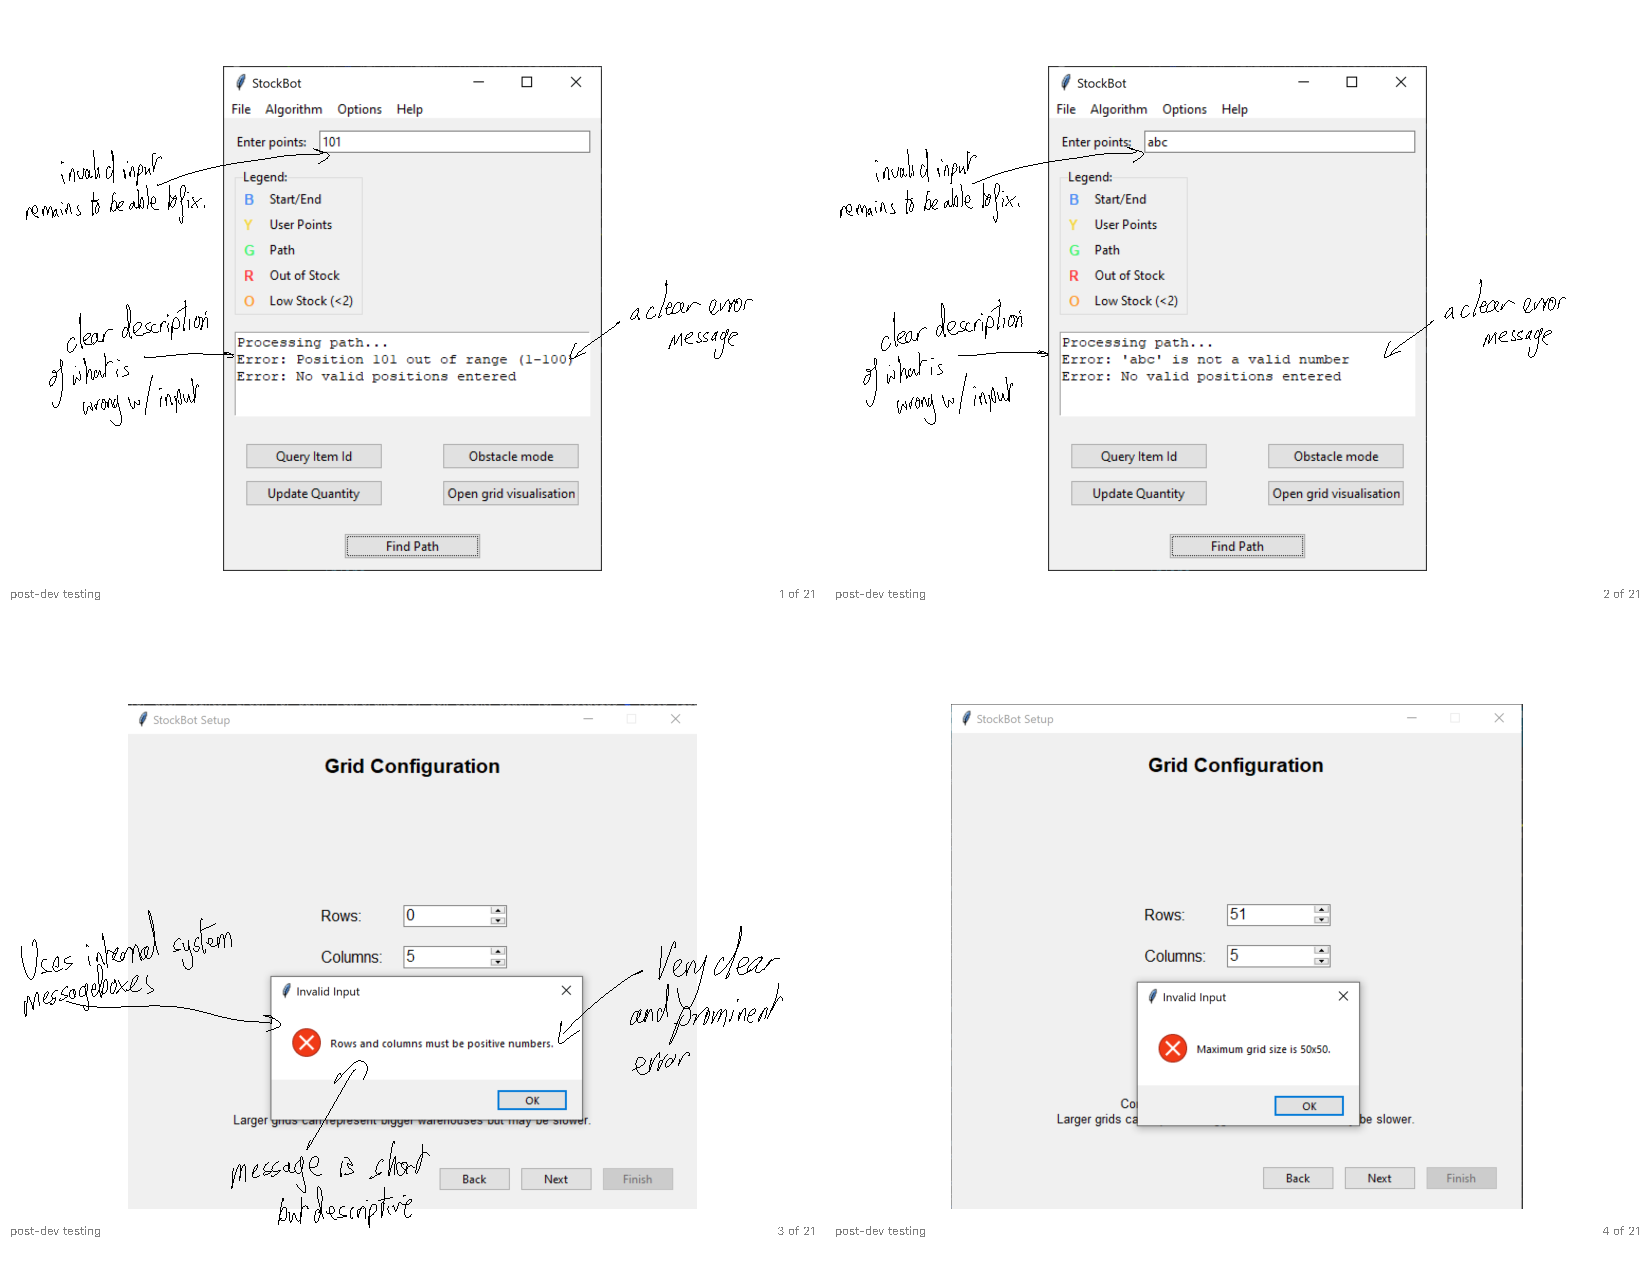
\includepdf[pages=-]{post-dev-testing/pdt.pdf}

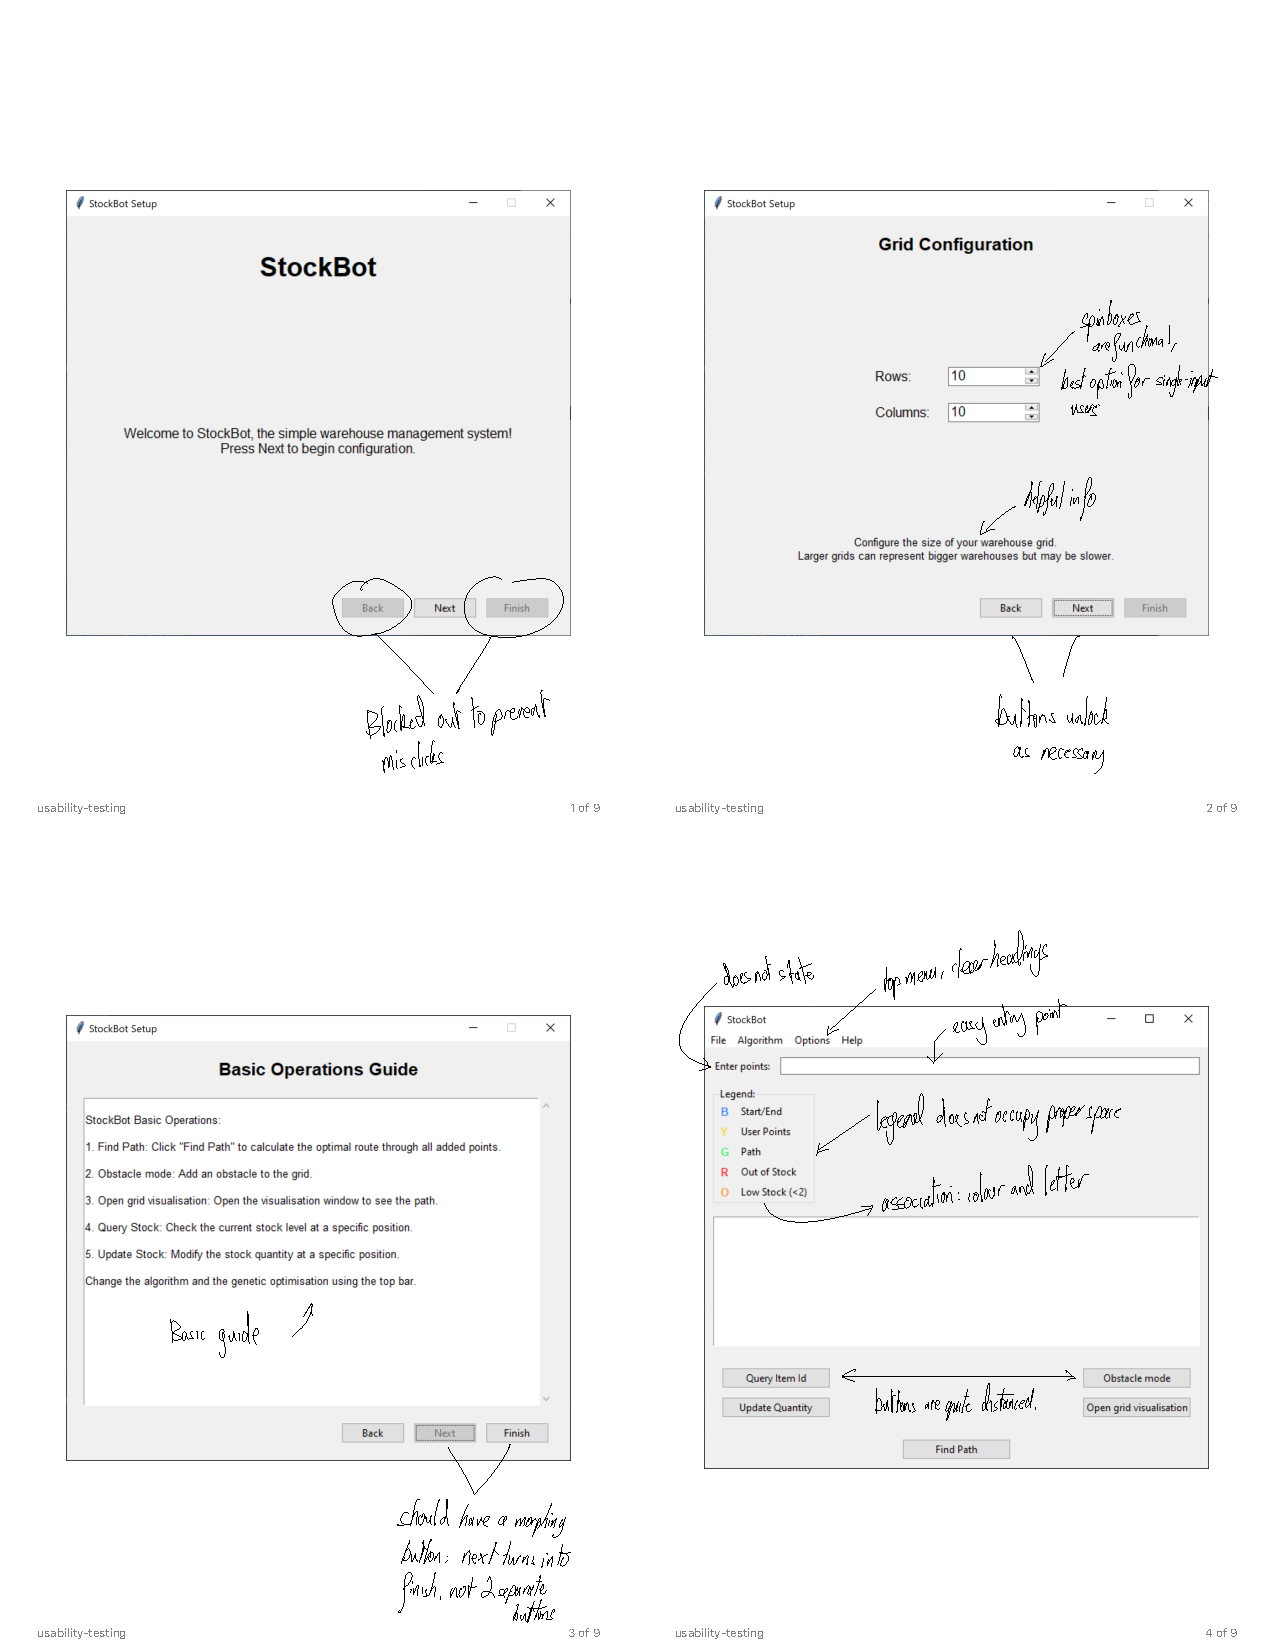
\includepdf[pages=-]{usability-testing-small.pdf}

% INSERT ANNOTATED PICS OF INTERFACE %  



\subsection{Comments}

\subsubsection{My evaluation}
Overall my solution is quite robust and usable, the validation is working excellently as you can see on the 1st and 2nd page with inputs having a range of data types and combinations. \newline Usability is good but definitely could be improved. Firstly, the buttons are quite spaced out in the main interface, which is something that could be fixed in future development. Next, the config screen has 3 buttons: Back, Next and Finish. In future, I should opt for 2 buttons so that it is easier to navigate.

\subsubsection{Stakeholder comments}

Your final prototype is very useful and usable. Overall I could see this being implemented with some GUI tweaks and a greater focus on performance. Well done!

\subsection{Link to success criteria}

My post-development tests tied in well with checking if I met my success criteria. The failed tests corresponded reasonably well with my success criteria, as the performance and rendering elements were not up to standard, reflected in the partial meeting of Criterion 10 and 17. See the next page for more details.
\newpage

%\newpage
\section{Success criteria revisited}

\begin{table}[htbp!]
	\centering
	\begin{tabularx}{\textwidth}{|c|X|X|}
		\hline
		\textbf{\#} & \textbf{Success Criterion} & \textbf{Justification} \\
		\hline
		1 & Displays the interface successfully with no errors & This makes sure the user can actually use the program's functions to their max ability. \\
		\hline
		2 & The system will identify and flag all items with stock levels below 2 units at the end of a run. & The threshold of 2 items provides a realistic simulation of a low-stock warning system. \\
		\hline
		3 & The pathfinding algorithm will calculate the optimal collection route in under 5 seconds for orders containing up to 10 items. & This is the most essential criterion: my stakeholder needs this solution to be fast. \\
		\hline
		4 & The system will reduce item collection time by 30-40\% compared to the manual method (baseline average: 7:31 minutes). & This is to prove that human-based list collection is inefficient compared to computational approaches. \\
		\hline
		5 & The application will run without crashes and minimal performance degradation for a minimum of 10 consecutive minutes during testing. & This demonstrates system stability \& reliability, which are required in any program. \\
		\hline
		6 & The system will successfully detect and navigate around 100\% of placed obstacles, while maintaining the high speed element as mentioned in Criterion 3. & Ensures the robot can adapt to changing warehouse conditions. \\
		\hline
		7 & The system will provide real-time position tracking with updates at least every 5 seconds and positional accuracy within 1 grid cell. & This is needed to ensure the solution can deploy on a larger scale and preventing issues. \\
		\hline
		8 & The stock verification system will prevent 100\% of attempts to locations with 0 inventory items. & Needed to improve efficiency and reduce time taken to process orders \\
		\hline
		9 & All system errors will be logged with detailed information including timestamp, error type, context, and affected component. & Error reporting is needed for troubleshooting and system improvement. \\
		\hline
		10 & The graphical user interface will respond to all user interactions within 2 seconds under normal operating conditions. & Responsive UI is critical for quick access to the program, since the main objective is to speed up operations. \\
		\hline
		11 & The system will successfully process and complete 95\% of assigned collection tasks without human intervention. & Measures the core functionality of autonomous performance of warehouse tasks and evaluating whether my solution is good enough. \\
		\hline
		12 & The system will provide collection completion estimates accurate to within $\pm$15\% of actual completion time for 90\% of tasks. & This addresses a request from my stakeholders for feedback throughout the pathfinding and collection process \\
		\hline
		13 & The application will successfully connect to and query the SQLite database with an overall response time not exceeding 1 second. & Efficient database operations are required for quick stock checking, this is the most likely place for a bottleneck. \\
		\hline
		14 & The path calculation algorithm will optimise routes to reduce total travel distance by at least 25\% compared to sequential collection. & Another measure of the effectiveness of the shortest path algorithm, but less important than time. \\
		\hline
		15 & The system will ensure all calculated paths use only orthogonal movements (up, down, left, right) and avoid diagonal navigation. & Models the layout of a warehouse, as you cannot cross items to reach others. \\
		\hline
		16 & The system will reject invalid inputs, such as non-existent points (e.g., Point 101 in a 10×10 grid) or malformed data (e.g., "abc"), with clear error messages. & Ensures the program is robust and does not fail, accounting for most if not all inputs \\
		\hline
		\end{tabularx}
		\end{table}
		\newpage
		\begin{table}[htbp]
		\centering
		\begin{tabularx}{\textwidth}{|c|X|X|}
		\hline
		\textbf{\#} & \textbf{Success Criterion} & \textbf{Justification} \\
		\hline
		17 & The system will maintain stable memory usage during continuous operation for up to 10 minutes, without exceeding a 15\% increase from baseline. & Measures the footprint and performance of the program; it is focused on speed, but it must also be reasonably memory-efficient. \\
		\hline
		18 & The system will recover gracefully from configuration errors (e.g., corrupted JSON files) by rejecting the invalid configuration and maintaining the previous state. & This is a fail-safe to ensure data is preserved and does not damage the current operating state. \\
		\hline
		19 & The system will return the stock level of any queried item within 1 second, regardless of grid size or database load. & Ensures the database is responsive enough. \\
		\hline
	\end{tabularx}
\end{table}

\subsubsection{Criterion 1:}
I have fully met this criterion because the interface displays flawlessly, there are no issues with the GUI and it is fully responsive.

\subsubsection{Criterion 2:}
I have fully met this criterion because the program flags all items with less than 2 items with a bold orange highlight, and this behaviour worked consistently.

\subsubsection{Criteria 3 and 4:}

I have fully met these criteria: all pathfinding took less than 1.2 seconds, see below for the measurements:

\begin{table}[h!]
	\centering
	\begin{tabularx}{\textwidth}{|c|c|c|X|}
		\hline
		Test Case & Graph Size (Nodes) & Intermediate Points & Time (seconds, 2dp) \\
		\hline
		1         & 400                & 2                   & 0.35              \\
		\hline
		2         & 400                & 2                   & 0.48              \\
		\hline
		3         & 400                & 2                   & 0.42              \\
		\hline
		4         & 400                & 2                   & 0.53              \\
		\hline
		5         & 400                & 5                   & 0.68              \\
		\hline
		6         & 400                & 5                   & 0.89              \\
		\hline
		7         & 400                & 5                   & 0.76              \\
		\hline
		8         & 400                & 5                   & 1.00              \\
		\hline
		9         & 400                & 10                  & 1.05              \\
		\hline
		10        & 400                & 10                  & 0.98              \\
		\hline
		11        & 400                & 10                  & 1.11              \\
		\hline
		12        & 400                & 10                  & 0.87              \\
		\hline
	\end{tabularx}
\end{table}

These times are significantly less than their human counterparts, making this a success.

\subsubsection{Criterion 5:}

I have fully met this: the program had no stability issues and I believe my program is robust enough to last a much longer time without crashes.

\subsubsection{Criterion 6:}

This criterion was fully met: the obstacle avoidance worked very well and in all cases either a path was found or the user was informed there was no valid path. Speed was minimally affected by this, too low a value to be of significance.

\subsubsection{Criterion 7:}

This criterion was NOT met: I did not implement any form of positional tracking due to time constraints. If I had enough time, I would add a path animation on the visualisation, with alternating colours depending on the action. This system would be easy enough to implement while still being intuitive.

\subsubsection{Criterion 8:}
This criterion was fully met: all items with no stock were avoided successfully, even with larger warehouses and more complex paths.
\subsubsection{Criterion 9:}

This criterion was PARTIALLY met. While I did have a logging system to track each stage of the process, errors would not be saved in the log, but would be saved in the terminal. In the future, I would use the same method of redirecting terminal output using sys as I did in development to save the error and gracefully shut down the program.

\subsubsection{Criterion 10:}

This criterion was PARTIALLY met. The interface was very responsive for all warehouses under 15x15, but getting larger it did struggle and often took 5+ seconds to recover after pressing the Find Path button. In this case, I would find a way to reimplement threading, as I did not have enough time to reimplement it. This would allow the GUI to run independent of other processes like pathfinding, increasing overall performance.

\subsubsection{Criterion 11:}

This criterion was fully met. In the final solution, >95\% of tasks required no intervention on my part.

\subsubsection{Criterion 12:}

This criterion was NOT met. I did not include approximate collection times as my main focus was finding the shortest path and due to time constraints I did not get a chance to simulate an actual robot, hence I did not incorporate collection time estimates. In the future, I would use an average of times taken to calculate the same path to provide ETCs - this would update each time it was run and then get more accurate as time went on.

\subsubsection{Criterion 13:}

This criterion was fully met. I successfully connected to the database and wrote sample, random data on each run, which was rapid and definitely quick enough for my stakeholders.

\subsubsection{Criterion 14:}

This criterion was fully met. The SPAs found a much shorter path than sequential collection on all occasions. This is due to the fact I simulated this as a travelling-salesman problem, hence the SPAs would at worst come up with an equivalent solution and at best the optimal solution.


\subsubsection{Criterion 15:}
This criterion was fully met. I ensured that diagonal movements were impossible by defining fixed directions using the coordinate system, where 1 represented up/right and -1 represented down/left.

\subsubsection{Criterion 16:}

This criterion was fully met. My validation methods prevented any sort of invalid input, restricting all fields to positive integers. Errors were made clear in the output box on the interface.

\subsubsection{Criterion 17:}

This criterion was PARTIALLY met. While my program was overall stable in terms of memory, larger warehouses often caused spikes of up to 30\%. In future, I would use more efficient data structures with a lower space complexity, which would reduce memory overhead.

\subsubsection{Criterion 18:}

This criteria was NOT met. I did not have enough time to implement any sort of persistence. In the future, I would use JSON files to store information about the database, or use an alternative to SQL like MongoDB to store and transfer data more securely.

\subsubsection{Criterion 19:}

This criteria was fully met. The database was very responsive and requests rarely took longer than 500ms, even for larger warehouses.

\section{Limitations}

My main limitation when developing my solution was time. I missed out on creating some quality-of-life features that would have made the solution even better. I mainly focused on getting core functionality working to a good-enough standard, and in the end my stakeholder was happy with the final result. Below are the features I would have implemented given the time and how I would approach them in the future:

\subsubsection{Direct feedback}

For this, I would have developed a function that would trace out the path as the 'robot' traversed it, with colours meaning different statuses. This would be an intuitive and easy way to check the status of the order, while not cluttering the UI with constant updates that would have come with a text-based approach. 

\subsubsection{Environment persistence}

For this feature, I would have used Python's JSON library to save all the database data to a universal format, and import that data in the same manner. I would have saved critical aspects first, like the warehouse configuration, before saving the database contents in a similar form to a SQL database, or would have saved the raw data and made a helper function to decode and reconstruct it.

\subsubsection{Path export}

This was not on the original plan for features, but I felt I should include it as a fallback. In the case where this software is used not autonomously but manually, it might be useful to export the visualisation of the path as an image, as it could show an employee where and how to walk to achieve the quickest route. To make this, I would use the pillow library from the Python package repository, and capture the window as a screenshot. I would then add a file dialog to allow the user to save the image to a location of their choice.

\section{Maintenance}

Maintenance features are mainly benefits of making my project with OOP principles. However, I did include some more maintenance features like detailed comments, clear naming and separation of concerns (splitting my code into respective files). This allowed me during development to build a good foundation, especially when I migrated from a CLI to a GUI. 

In terms of future maintenance, I could add a feature into the top menus that fetches the latest version from GitHub, keeping the version up to date as the software progresses. This would be accompanied by an installer function which would check and install any dependencies required by the new version. This would probably be done through PIP: the python package manager: it allows dependencies to be listed in a file and automatically installed in one command.

I would also set up a feedback system on a task-tracking software like Linear, which allows future testers to flag features, bugs and other issues they may encounter. This could be directly built into the software - a bug tracker that could automatically send a bug report to me through APIs.